\documentclass{beamer}
\usetheme{Boadilla}
\usepackage{tikz}

\title{Weekly Presentation}
\subtitle{Week 37}
\author{Martin Blaszczyk}
\institute{Luleå University of Technology}
\date{\today}

\begin{document}
\begin{frame}
    \titlepage
\end{frame}

\begin{frame}
    \frametitle{Overview}
    \tableofcontents
\end{frame}
%%%%%%%%%%%%%%%%%%%%%%%%%%%%%%%%%%%%%%%%%%%%%%%%%%%%%%%%%%%%%%%%
%%%%%%%%%%%%%%%%%%%%% Project Structure %%%%%%%%%%%%%%%%%%%%%%%%
%%%%%%%%%%%%%%%%%%%%%%%%%%%%%%%%%%%%%%%%%%%%%%%%%%%%%%%%%%%%%%%%
\section{Project structure}
\begin{frame}
    \subsection{Group members}
    \frametitle{Group members }
    \begin{itemize}
        \item Y-students
        \begin{itemize}
            \item Martin Blaszczyk - Project leader and object detection
            \item Edward Cedergård - Gripping tool
            \item Niklad Dahlqvist - Gripping tool
            \item Måns Norell - Movable base
        \end{itemize}
        \item D-students
        \begin{itemize}
            \item Edward Källstedt - Object detection
            \item Albin Martinsson - Arrowhead and Git
        \end{itemize}  
    \end{itemize}
\end{frame}
%%%%%%%%%%%%%%%%%%%%%%%%%%%%%%%%%%%%%%%%%%%%%%%%%%%%%%%%%%%%%%%%
%%%%%%%%%%%%%%%%%%%%%%%% Meetings %%%%%%%%%%%%%%%%%%%%%%%%%%%%%%
%%%%%%%%%%%%%%%%%%%%%%%%%%%%%%%%%%%%%%%%%%%%%%%%%%%%%%%%%%%%%%%%
\begin{frame}
    \subsection{Meetings}
    \frametitle{Meetings}
    Apart from the planned meetings there will be planned \textit{lab sessions} in
    the project room. 
    \\~\
    \begin{columns}

        \begin{column}[]{0.5\textwidth}
            \textbf{Monday meetings}
            \begin{itemize}
                \item Status update
                \item Qustions for the seminar
                \item Gameplan for the seminar
            \end{itemize}
        \end{column}

        \begin{column}[]{.5\textwidth}
            \textbf{Tuesday meetings}
            \begin{itemize}
                \item Feedback review
                \item Group feedback
                \item Gameplan for the coming week
            \end{itemize}
        \end{column}

    \end{columns}
\end{frame}

%%%%%%%%%%%%%%%%%%%%%%%%%%%%%%%%%%%%%%%%%%%%%%%%%%%%%%%%%%%%%%%%
%%%%%%%%%%%%%%%%%%%%%%%% Time Plan %%%%%%%%%%%%%%%%%%%%%%%%%%%%%
%%%%%%%%%%%%%%%%%%%%%%%%%%%%%%%%%%%%%%%%%%%%%%%%%%%%%%%%%%%%%%%%
\begin{frame}
    \subsection{Time plan}
    \frametitle{Overall timetable}
    \begin{table}
        \begin{tabular}{| l | c | c | c | c }
            
            Sep & Oct & Nov & Dec \\
            \hline \hline
            Concept generation & Evaluation & Evaluation &  \\ 
            \hline
            Theory & Prototyping & Evaluation & Finishing up \\
            \hline
            Simulation & Evaluation & Evaluation & \\
            \hline
            Prototyping & Final Design & Evaluation &  \\
            \hline
 
        \end{tabular}
    \end{table}    
\end{frame}


\begin{frame}
    \frametitle{Time plan for September}
    \begin{table}
        \begin{tabular}{l | c | c | c | c }
        Subproject & Week 1 & Week 2 & Week 3 & Week 4 \\
        \hline \hline
            Arrowhead & Reading& Setup & API & Prototyping\\
            Movable base & Reading& Modeling & Simulation & Implementation\\
            Arm and grip  & Reading & Kinematics & Simulation& Prototyping\\
            Object detection & Reading & Testing & Prototyping & Evaluation\\
        \end{tabular}
    \end{table}
\end{frame}

\begin{frame}
    \frametitle{Github}
    Git is a great way to structure and sync a project. With commits it's easy to 
    "backup" the code in case something goes wrong. All members will be able to 
    have an insight into the project nad help eachother. Not all group members
    have used Git extensively so there's a learning curve in the beginning and how 
    to structure the repo in a good way. 
    \\~\
\end{frame}

\begin{frame}
    \frametitle{Github - branches}
    \begin{itemize}
        \item Master and development branch.
        \item Separate branch for each part of the project.
        \item Proofreading of the report by two people before it ends up in master.
        \item Code review by the other team members before it ends up in master. 
    \end{itemize}  
\end{frame}

\begin{frame}
    \frametitle{Github - issues}
    \begin{itemize}
        \item Tasks
        \item Assingees and mentions
        \item Labels
        \item Milestones
    \end{itemize}  
\end{frame}

%%%%%%%%%%%%%%%%%%%%%%%%%%%%%%%%%%%%%%%%%%%%%%%%%%%%%%%%%%%%%%%%%%%%%%%%%%
%%%%%%%%%%%%%%%%%%%%%%%%%%%% Engineering Problem %%%%%%%%%%%%%%%%%%%%%%%%%
%%%%%%%%%%%%%%%%%%%%%%%%%%%%%%%%%%%%%%%%%%%%%%%%%%%%%%%%%%%%%%%%%%%%%%%%%%
\section{Engineering problem}
\begin{frame}
    \subsection{Idea generation}
    \frametitle{Idea generation} 
    \begin{itemize}
        \item A common picture
        \item Requirements
        \item Idea generation in subgroups
        \item Prototype and evaluation\\~\
    \end{itemize} 

    The concept generation phase is an ongoing process so after evaluation
    some adjustments will be done depending on the performance
    of the design.
\end{frame}

\begin{frame}
    \subsection{Litterature}
    \frametitle{Litterature}

    \begin{columns}
        \begin{column}[]{0.5\textwidth}
            \textbf{Robotics, Vision \& Control }\\
            \textit{Robert Corke}
            \begin{itemize}
                \item Gives s good overview
                \item Covers most topics
                \item Good code examples\\~\
            \end{itemize}
            \textbf{Robot Dynamics \& Control}\\
            \textit{Mark W. Spong}
            \begin{itemize}
                \item Popular in robotics
                \item More focused on the theory
                \item Covers basic robotic kinematics
            \end{itemize}

        \end{column}
        
        \begin{column}[]{.5\textwidth}
            \textbf{Programming Robots with ROS}
            \textit{Morgan Quigley}
            \begin{itemize}
                \item Good for beginners
                \item Explains most basic parts of ROS \\~\
            \end{itemize}
            \textbf{Arrowhead Git}
            \begin{itemize}
                \item Official documentation
            \end{itemize}
        \end{column}
        

    \end{columns}
\end{frame}

\begin{frame}
    \subsection{Requirements}
    \frametitle{Concept evaluation}
    Each part of the project has requirements to keep the project focused 
    on the task. During the evaluation phase the concepts will have to achive
    the requirements which are considered \textit{bare minimum}. 
\end{frame}

\begin{frame}
    \frametitle{Robotic arm requirements}
    \begin{itemize}
        \item Move the arm/claw to a specific coordinate in space
        \item Have 4 degrees of freedom in front of the robot.
        \item Detect if the object is grabbed
        \item Able to hold a object shape as a cylinder
        \item Pick up object if dropped during path*
    \end{itemize}
\end{frame}

\begin{frame}
    \frametitle{Movable base}
    \begin{itemize}
        \item Move to a certain point in space
        \item Overcome the factory platform
        \item Line up and angle correctly so that the robot arm can reach an object
    \end{itemize}
\end{frame}

\begin{frame}
    \frametitle{Object detection}
    \begin{itemize}
        \item Given a distinctly colored line along the floor be able to track it and
        feed back an accurate measurement of how much the robot deviates from said line.
        \item Camera input should be filterable by RGB pixel values.
        \item The system should be able to recognize and read of QR Codes.
        \item It should be possible for the system to keep up with and process a continuous video stream in real-time.
        \item An accompanying GUI should exist where the raw video stream can be seen adjacent to a video stream where detection is active.
        \item Feed position data to the other systems
    \end{itemize}
\end{frame}

\begin{frame}
    \frametitle{Arrowhead}
    \begin{itemize}
        \item Have a raspberry pi as a plant, giving the robot a clear directive that the piece is ready for pick up.
        \item Have authorized communication between the robot and the plant.
        \item Being able to detect if the piece is ready for pick up or not using a distance sensor at the end
        of the conveyor belt.
        \item The robot should be able to tell the plant if the piece is not picked up properly.
        \item The robot should be able to tell the plant after a succesfull pick up.
    \end{itemize}
\end{frame}

\subsection{Flow charts}
\begin{frame}
    \frametitle{General flow}
    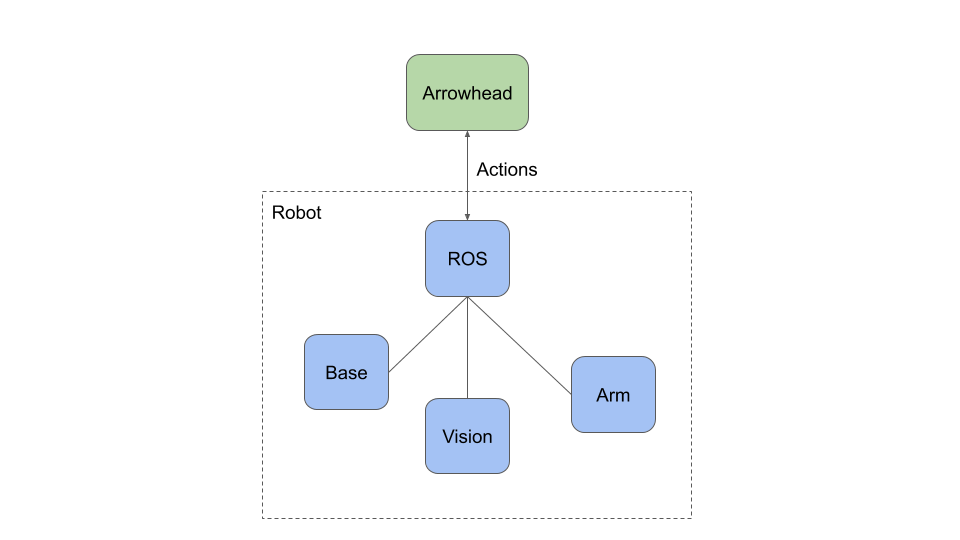
\includegraphics[width=\textwidth]{img/general_flow.png}
\end{frame}

\begin{frame}
    \frametitle{Moving base flow}
    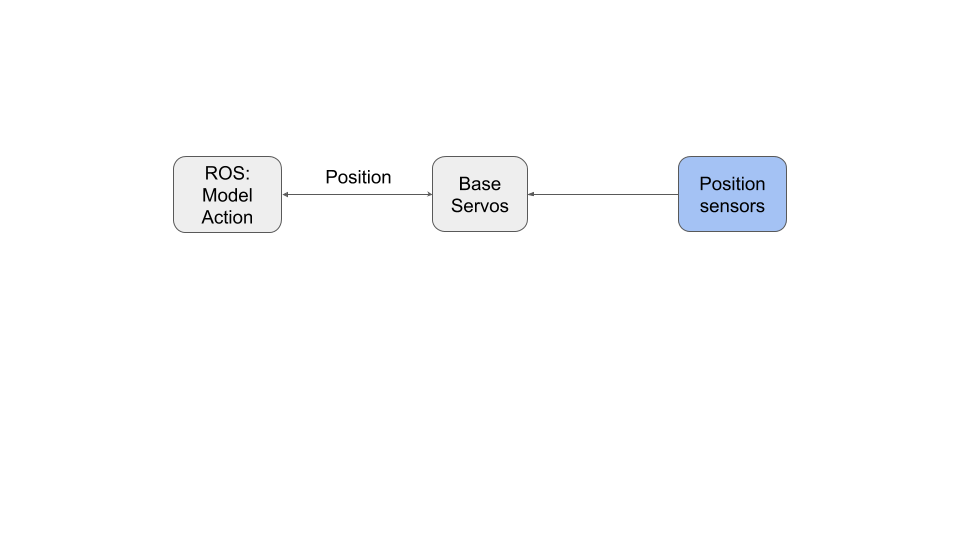
\includegraphics[width=\textwidth]{img/base_flow.png}
\end{frame}

\begin{frame}
    \frametitle{Robotic arm flow}
    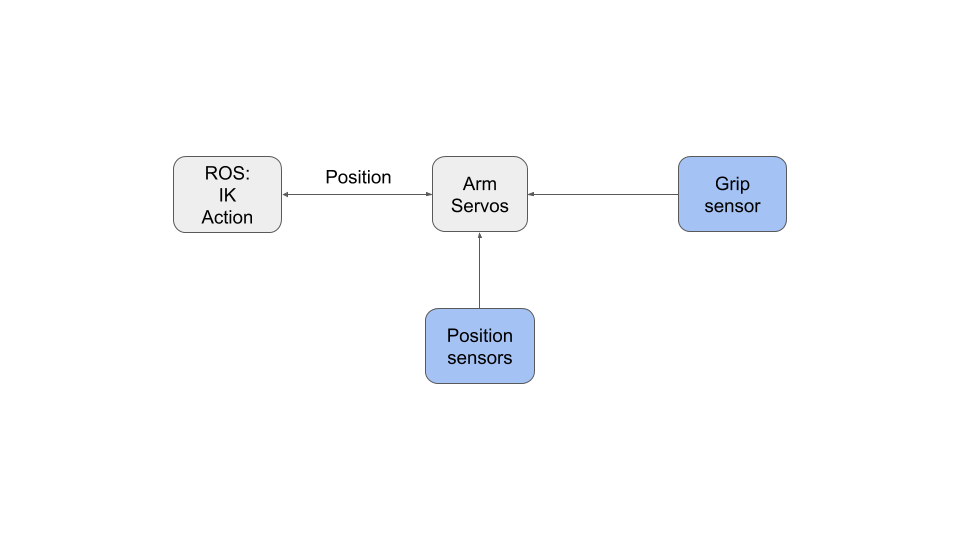
\includegraphics[width=\textwidth]{img/arm_flow.png}
\end{frame}

\begin{frame}
    \frametitle{Object detection flow}
    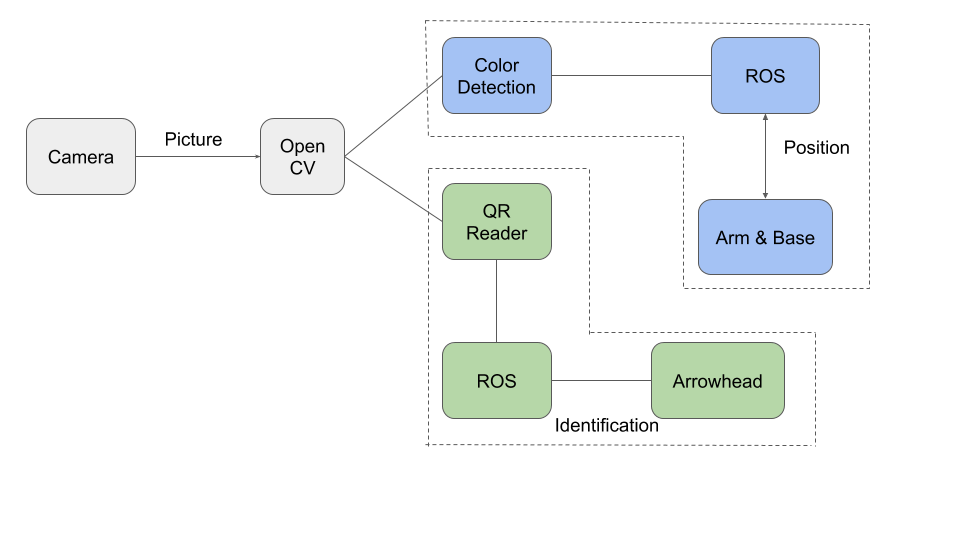
\includegraphics[width=\textwidth]{img/vision_flow.png}
\end{frame}


\begin{frame}
    \frametitle{Challenges / Unknowns}
    \begin{itemize}
        \item Processing power
        \item Complexity
        \item Hardware failures
        \item Losing focus 
    \end{itemize}
\end{frame}

\begin{frame}
    \begin{center}
        \Huge Questions?
    \end{center}
\end{frame}



\end{document}